% !TEX TS-program = pdflatex
% !TEX encoding = UTF-8 Unicode

% This is a simple template for a LaTeX document using the "article" class.
% See "book", "report", "letter" for other types of document.

\documentclass[11pt]{article} % use larger type; default would be 10pt

\usepackage[utf8]{inputenc} % set input encoding (not needed with XeLaTeX)

%%% Examples of Article customizations
% These packages are optional, depending whether you want the features they provide.
% See the LaTeX Companion or other references for full information.

%%% PAGE DIMENSIONS
\usepackage{geometry} % to change the page dimensions
\geometry{letterpaper} % or letterpaper (US) or a5paper or....
\geometry{margin=1in} % for example, change the margins to 2 inches all round
% \geometry{landscape} % set up the page for landscape
%   read geometry.pdf for detailed page layout information

\usepackage{graphicx} % support the \includegraphics command and options

% \usepackage[parfill]{parskip} % Activate to begin paragraphs with an empty line rather than an indent

%%% PACKAGES
\usepackage{booktabs} % for much better looking tables
\usepackage{array} % for better arrays (eg matrices) in maths
\usepackage{paralist} % very flexible & customisable lists (eg. enumerate/itemize, etc.)
\usepackage{verbatim} % adds environment for commenting out blocks of text & for better verbatim
\usepackage{subfig} % make it possible to include more than one captioned figure/table in a single float
% These packages are all incorporated in the memoir class to one degree or another...
\usepackage{wrapfig}
\setlength{\columnsep}{15pt}
\setlength{\intextsep}{0pt}

\usepackage{fancyvrb}
\usepackage{hyperref}

%%% HEADERS & FOOTERS
\usepackage{fancyhdr} % This should be set AFTER setting up the page geometry
\pagestyle{fancy} % options: empty , plain , fancy
\renewcommand{\headrulewidth}{0pt} % customise the layout...
\lhead{}\chead{}\rhead{}
\lfoot{}\cfoot{\thepage}\rfoot{}

%%% SECTION TITLE APPEARANCE
\usepackage{sectsty}
\allsectionsfont{\sffamily\mdseries\upshape} % (See the fntguide.pdf for font help)
% (This matches ConTeXt defaults)

%%% ToC (table of contents) APPEARANCE
\usepackage[nottoc,notlof,notlot]{tocbibind} % Put the bibliography in the ToC
\usepackage[titles,subfigure]{tocloft} % Alter the style of the Table of Contents
\renewcommand{\cftsecfont}{\rmfamily\mdseries\upshape}
\renewcommand{\cftsecpagefont}{\rmfamily\mdseries\upshape} % No bold!

%%% END Article customizations

%%% The "real" document content comes below...

\title{REMUS \underline{S}ynthetic \underline{A}perture \underline{OV}e\underline{R}ride (SAOVR) Documentation \\ Version 1.1}
\author{Tom Dodson \\ Dept. of Physics and Astronomy \\ University of Pennsylvania \\ \href{tcdodson@gmail.com}{tcdodson@gmail.com}
 \\ 859-866-3365}
\date{} % Activate to display a given date or no date (if empty),
         % otherwise the current date is printed 

\begin{document}
\maketitle

\section{SAOVR Internal Operations}
\subsection{Overview}
The SAOVR program runs continuously on the AUV's PC stack, which runs Windows XP. The package uses the Windows API to handle threading, and the Hydroid RECON interface to interact with the vehicle.
In broad terms, the task of the SAOVR software package is as follows:

\begin{enumerate}
\item Provide a keep-alive message (Section \ref{sec:keepalive}), allowing the vehicle to execute the mission programmed via VIP
\item Wait for an acoustic tag signal via MapHost file (as described in Sections \ref{sec:tagfile} and \ref{sec:startup}).
\item If a tag is heard, invoke a full override (\texttt{\#E}), as specified by the RECON protocol (see pp. 1, 35 of the RECON documentation).
\item Execute the synthetic aperture specified for the given tag.
%TODO
\item At the end of the override aperture, release control of the vehicle. The vehicle will then return to the nearest point on the trackline 
	(note that this is not the default behavior -- see pp. 2, 43 of the RECON documentation) and resume the pre-programmed mission.
\item After all appropriate cooldowns (Section \ref{sec:cooldowns}) have expired, return to step 1.
\end{enumerate}

\subsection{The Keep-Alive Message}
\label{sec:keepalive}
In order for the vehicle to operate, it must receive a keep-alive message at least every 5 seconds (see RECON documentation, p. 33). This keep-alive 
message may either be a \mbox{\texttt{\#C}} command or a \mbox{\texttt{\#v}} command, and is usually provided by the REMUS External Control 
program. The REMUS SAOVR program must take over this responsibility, and sends either a version command (when not in override mode), 
or a depth command (when in a full override) every 2 seconds.  This allows the software to miss a single message (due to, for example, inability to
acquire the COM port mutex) while still allowing the vehicle to operate, so long as it does not miss two messages in a row.

\subsection{Cooldowns}
\label{sec:cooldowns}
In order to prevent the vehicle from executing overrides \textit{ad infinitum}, the system implements two types of cooldowns - a global cooldown and
a tag-specific cooldown. The first timer is started when any override is executed, and the second, independent, timer is started when the associated tag is heard. When the global
cooldown is active, all tags are ignored. When the tag-specific cooldown is active, that only the associated tag code is ignored. 
For further details, see Section \ref{sec:cooldown_example}.

\subsection{Start-up Algorithm}
\begin{enumerate}
\item Opens the log file and begin writing.
\item Opens COM1 to the RECON stack.
\item Opens the \texttt{tag\_file.txt} lookup table.
\item Parses the tag file, line by line, reading in the appropriate command files, and writing them back out to the log. The latter operation gives the 
	user an opportunity to sanity-check the programmed apertures before placing the vehicle in the water.
\item Waits for the the MapHost output \texttt{.csv} file to be created with the appropriate name and path, then starts the file watcher thread.
\item Starts the keepalive (TX) and status message reader (RX) threads.
\item The system is now ready, and will begin listening for tags as soon as it receives the `Mission Start' command.
\end{enumerate}




\section{File System Setup}
\label{sec:filesystem}

\begin{figure}[h]
\centering{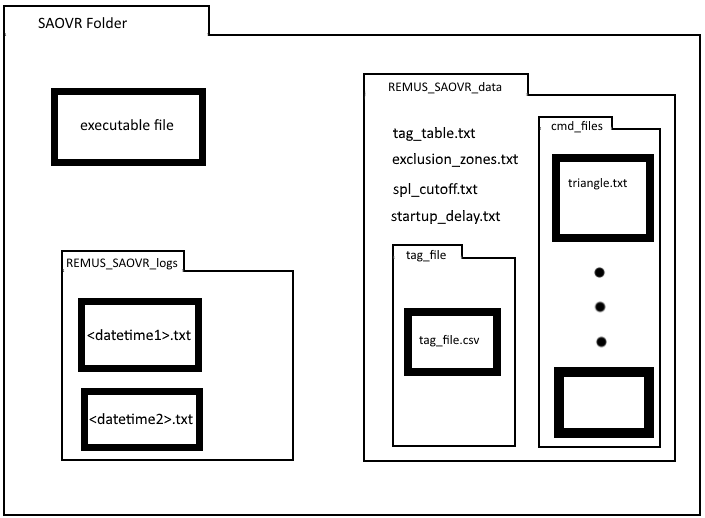
\includegraphics[width=\textwidth]{img/filesystem.png}}
\caption{The SAOVR filesystem layout}
\label{fig:filesystem}
\end{figure}


While the program does not require a dedicated folder, it is a good practice
to place the executable file (.exe) in it's own folder (see Figure \ref{fig:filesystem}). The program requires two folders in the same folder as the executable - a log folder and a data folder. 

\subsection{Log Files}

A log file is automatically created in the folder \mbox{\texttt{REMUS\_SAOVR\_logs}} each time the program is started. The new log file is named in a
\mbox{\texttt{YYMMDD\_hhmmss}} format. The log contains information about the run,  and the status of the REMUS is written out to the log file
roughly every 40 seconds.

The primary purpose of the log file is to store debugging information about any potential errors encountered during a run and to 
allow the user to reconstruct the apertures that are run during the mission.

\subsection{Data Folder}

The data folder, named \mbox{\texttt{REMUS\_SAOVR\_data}}, must be in place when the program is executed, or it will immediately abort. This folder
contains three critical components -- the tag table file, the command files (typically in their own folder), and the tag file (code list output from MapHost).

\subsubsection*{Startup Delay}
In order to facilitate uninterrupted vehicle startup, the SAOVR software
can be configured to ignore all overrides that would otherwise be triggered for a specified number of seconds after the vehicle is
commanded to start the mission.

The file containing the startup delay, \mbox{\texttt{startup\_delay.txt}},
is contained in the data folder, and contains a single integer number.
If the file is not found, the software will use the default value of
$60$ seconds.

No checks for input sanity are performed, so the log should be
scrutinized during setup. The minimum startup delay should be
taken to be $1$ second. Zero or negative numbers, in particular, will not trigger an error on startup, but are likely to cause unpredictable behavior.

No comments are allowed in this file.


\subsubsection*{SPL Cutoff}
The SAOVR software can be configured to trigger overridess only 
when tags above a 
certain SPL (sound pressure level) are heard. The default SPL cutoff is
30, the units of which are the same units as expressed in the 
MapHost CSV file output in the \textbf{Power} column.

The file containing the SPL cutoff, \mbox{\texttt{spl\_cutoff.txt}}, 
is contained in the data folder, and contains a single floating
point number. If the file is not found, the software
will proceed with the default cutoff ($30$). If a lower minimum is required
for a particular mission, the file must be present.

No checks for input sanity are performed, so the log should be
scrutinized during setup. While the minimum SPL cutoff should be
taken to be zero, negative numbers, in particular, are allowed,
and will likely result in accepting all tags as potential triggers
for overrides.

No comments are allowed in this file.

\subsubsection*{Exclusion Zones}

In order to avoid executing maneuvers in areas where a maneuver may put
the vehicle at risk of damage, the user has the ability to define
exclusion zones -- areas in which the vehicle will not respond to
any overrides that would otherwise be triggered.

The file, which is contained in the data folder and named
\mbox{\texttt{exclusion\_zones.txt}}, is formatted as below.

This file does not have to be present in order for the SAOVR
software to function. 

The exclusion zones will be output when the software starts.

\emph{TODO: put a graphic in this section.}

\begin{Verbatim}[xleftmargin=.5in,fontsize=\small,frame=single]
% Each line in this file has three whitespace delimited entries which
% specify a circle. The first two numbers are the latitude and longitude
% in the same format as the REMUS VIP software (decimal minutes).
%
%latitude		longitude		radius
58N22.479		134W40.437		200
\end{Verbatim}

\subsubsection*{Tag Table}

This file at must be placed in the data directory, and named \mbox{\texttt{tag\_table.txt}}. It contains first the global cooldown in seconds (an integer -- the
concept of cooldowns will be explained in a later section),
then at least one line beginning with a tag code (an integer) and either a path (absolute, or relative to the executable) or
the keyword \mbox{\texttt{IGNORE}}. 

The \mbox{\texttt{IGNORE}} keyword simply tells the software to completely ignore the given tag code. If, instead, a path is specified, it points to a 
command file which contains a description of the aperture to be run for the given tag code.
The tag code -1 is used to specify the default aperture, which will be executed for any tags not explicitly specified in this file. 
If no default is explicitly specified, the first command file (\emph{not} counting any  \mbox{\texttt{IGNORE}} lines) will be used as the default.

Any line beginning with \texttt{\%} is considered a comment, and the line will be ignored. See below for an example of the file.

\begin{Verbatim}[xleftmargin=.5in,fontsize=\small,frame=single]
% First line of this file is the global cooldown time in seconds, then each
% additional line is a tag ID (-1 means 'default') and an associated file
% describing the aperture to run (or the IGNORE command)
90

-1	REMUS_SAOVR_data\\cmd_files\\forwards_triangle.txt
10284	IGNORE
\end{Verbatim}

In this file, for example, the first three lines are comments, the global cooldown is set to 90 seconds, tage code 10284 will be ignored, and all other tags
will execute the aperture given by \mbox{\texttt{forwards\_triangle.txt}}

\subsubsection*{Command Files}

Command files hold the information needed to execute a synthetic aperture maneauver. Lines beginning with a \texttt{\%} are treated as comments
and ignored. The first entry in the file is an integer cooldown time, in seconds, for the aperture. 

Each leg of the aperture must contain exactly four entries, in a fixed order:
\begin{enumerate}
  \item A floating point number representing the length of the leg, in seconds. Note that a decimal point is not required, as integer numbers of seconds
  	will be interpreted correctly.
  \item The command \mbox{\texttt{>ALTER HEADING}}
	\footnote{Note that the \mbox{\texttt{>ALTER HEADING}} command is \emph{not} a part of the RECON protocol - it is a command that I 
	introduced in order to give users the ability to write arbitrary apertures without \textit{a priori} knowledge of the direction
	of the vehicle at the time of the override},
	followed by whitespace, followed by a floating point number. 
	The number given will be added
  	to the current heading of the vehicle and set as the heading goal for that leg. If the heading change is large, the time required for the vehicle to 
  	reach the new heading should be factored into the length of the leg.
  	
	The new heading is computed in the following way:
	\begin{Verbatim}[fontsize=\footnotesize]
	//add the current heading, the delta, then add 360 just to make sure it's a
	// positive number before taking the mod 360
	float new_heading = 
			fmod(get_current_heading() + alter_heading + 360.0, 360.0);
	\end{Verbatim}

  \item A depth command, without a checksum, as detailed by the RECON documentation, pp. 33-34. The depth command will be used as
  	the keepalive command for the duration of the leg (the keepalive concept is explained in Section \ref{sec:keepalive}).
  \item A speed conmand, without a checksum, as detailed by the RECON documentation, pp. 33-34. 
\end{enumerate}

Finally, the file must end with a \mbox{\texttt{>RELEASE TO NEAREST}} or \mbox{\texttt{>RELEASE TO START}} command
\footnote{Note that these commands are also not part of the RECON protocol -- the associated RECON command is \mbox{\texttt{\#c}}. } .
This tells the vehicle
whether to return to the nearest point on the programmed trackline, or to return to the position where the override was 
initiated (see Figure \ref{fig:return}).
Note that the latter behavior is the default vehicle behavior (see page 9 of the RECON documentation).

Since each leg must have exactly four entries, if one does not wish to change the depth or speed between legs, the depth and 
speed commands must be
duplicated between legs. Below is an example command file, \mbox{\texttt{forwards\_triangle.txt}}, which runs a 20m 
equilateral triangle aperture, then
returns to the nearest point on the trackline (see Figure \ref{fig:fwd_triangle}).


\begin{figure}[hb]
\vspace{22pt}
\centering
\captionsetup{width=.6\linewidth}
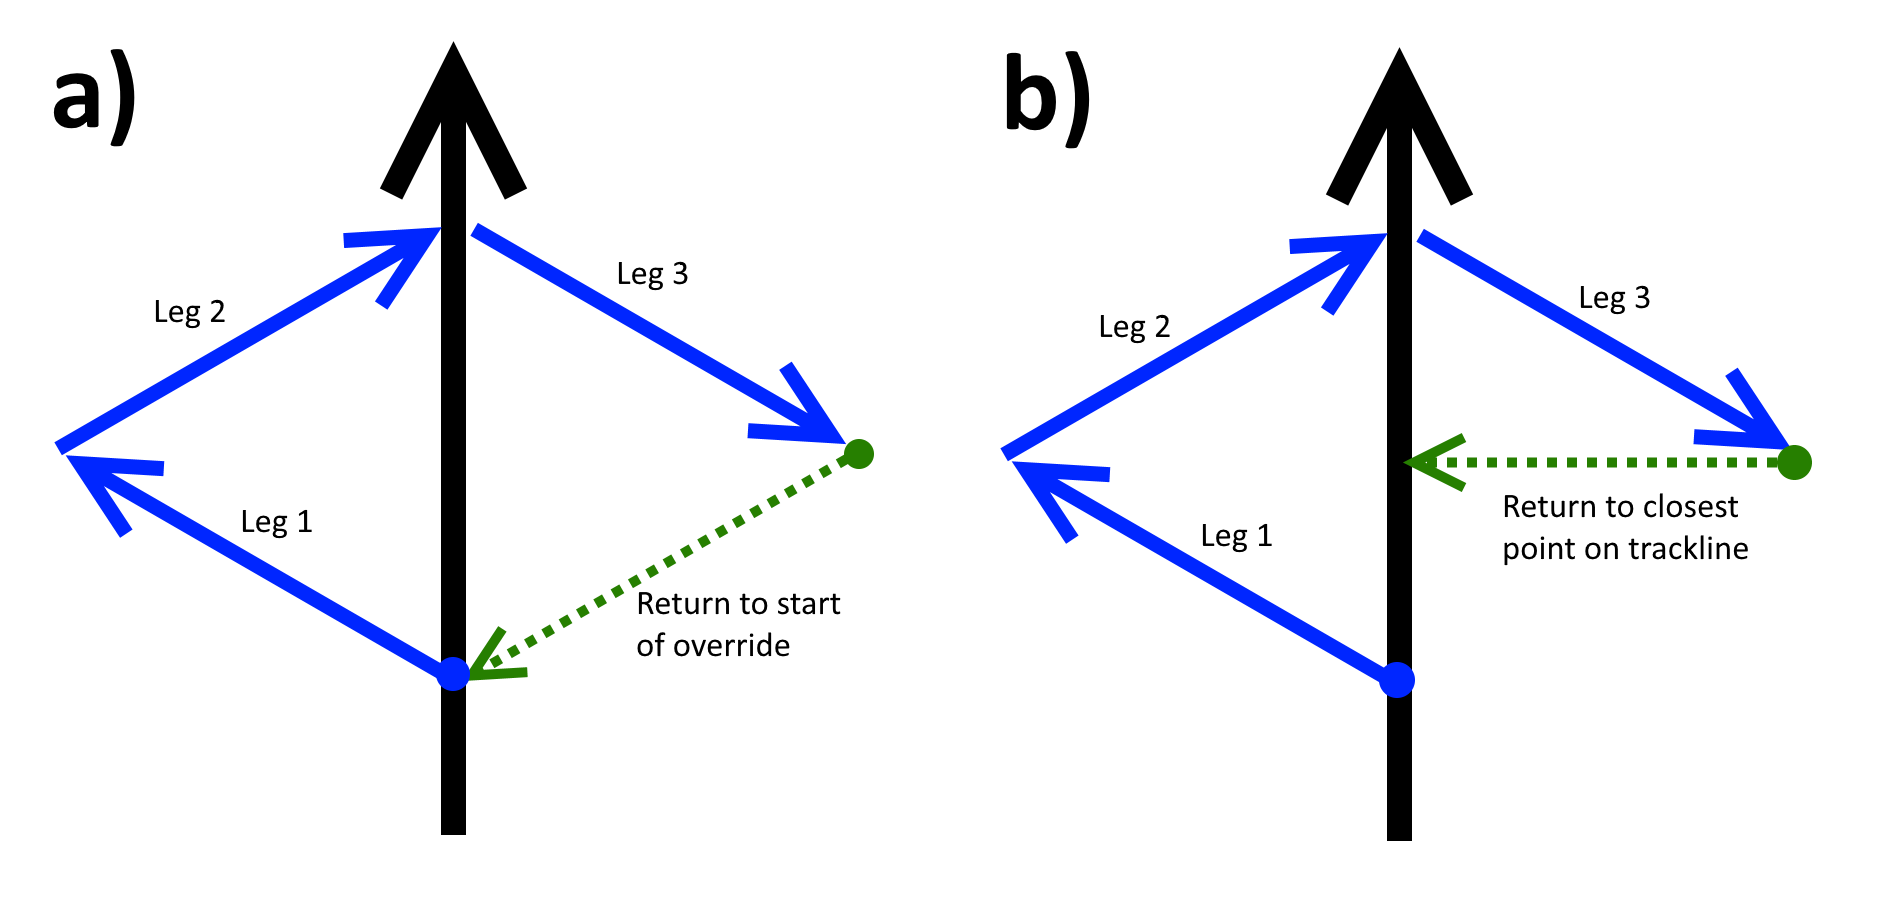
\includegraphics[width=0.8\textwidth]{img/return_behavior.png}
\caption{Possible behaviors of the REMUS when override is released (green dot). Note that a) is the default vehicle behavior.}
\label{fig:return}
\vspace{22pt}
\end{figure}


\begin{Verbatim}[xleftmargin=.5in,fontsize=\small,frame=single]
%Cooldown period for this particular aperture, in seconds
120

%Turn to make the first half-leg of the triangle (90 deg)
% 1.8 knots = 0.926 m/s, so 10 meters requires 10.8s
10.8
>ALTER HEADING 90
#C,Depth,Altitude,30.0
#C,Speed,1.8 knots

%Turn to make the second leg of the triangle (-120 deg)
%10 meters requires 22.5s
22.5
>ALTER HEADING -120
#C,Depth,Altitude,30.0
#C,Speed,1.8 knots

%Turn to make the third leg of the triangle (-120 deg)
22.5
>ALTER HEADING -120
#C,Depth,Altitude,30.0
#C,Speed,1.8 knots

%Turn to finish the first half-leg of the triangle (-120 deg)
10.8
>ALTER HEADING -120
#C,Depth,Altitude,30.0
#C,Speed,1.8 knots

%Release the override and let the vehicle return to
% the nearest point on the trackline (which should be nearby), 
% completing the triangle
>RELEASE TO NEAREST
\end{Verbatim}

\begin{figure}[t]
\centering
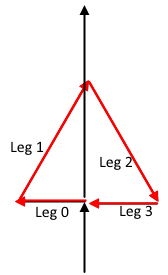
\includegraphics{img/fwd_triangle.png}
\caption{Forwards triangle aperture}
\label{fig:fwd_triangle}
\end{figure}

\subsubsection*{Tag File}
\label{sec:tagfile}

This file must be placed in the data directory, in a subdirectory named \mbox{\texttt{tag\_file}}, and named \mbox{\texttt{tag\_file.csv}}. It is the code 
output file from MapHost, and the SAOVR software will wait to begin execution until it finds the file. The file looks like the short example given below:

\begin{Verbatim}[xleftmargin=.5in,fontsize=\small,frame=single]
ID,Data,Power,Time,dd/mm/yy
10284,,59, 17:06:33.11271,05/04/15
15777,,99, 17:06:50.52188,05/04/15
\end{Verbatim}

For now, only the first comma-separated entry, the tag code, is used by the software. The power levels and timestamps may, in the future, be used to
program \emph{adaptive} synthetic apertures, but this feature has not yet been implemented.





\section{Operational Examples}
\subsection{Cooldowns}
\label{sec:cooldown_example}
\subsubsection*{Example 1}
Assume a 120 second global cooldown. Codes 42, 101, 102, and 103 are in the water. Code 42 is set to \mbox{\texttt{IGNORE}}, while code 101 has an
aperture with a runtime of 40 seconds, and a cooldown of 60 seconds. Since no default aperture is specified, the aperture for code 101 is assumed to be
the default.
\\


\begin{tabular}{|r||l|c|}
\hline
t (seconds) & Event & Tags currently ignored\\
\hline
0 & Vehicle hears tag 101, software begins override & 42\\
40 & Software releases override &  42,101,102,103\\
60 & Tag 101 override expires, but global override still active & 42,101,102,103\\
120 & Global override expires & 42\\
\hline
\end{tabular}

\subsubsection*{Example 2}
This example is meant to demonstrate that the cooldowns are handled \emph{per code}, even when the default aperture is executed, and also
demonstrates how queueing of codes is handled (i.e. the queue size is one -- only the last tag heard during an override is remembered).

Assume a 30 second global cooldown. Codes 101, 102, and 103 are in the water. Code 101 has an
aperture with a runtime of 20 seconds, and a cooldown of 30 seconds. The default aperture has a 40 second runtime and a 60 second cooldown.
\\

\begin{tabular}{|r||l|c|c|c|c|}
\hline
 & & \multicolumn{4}{|c|}{Cooldown time remaining} \\
\hline
t (seconds) & Event & global & 101 & 102 & 103 \\
\hline
0 & Hear code 103, enter override & 30 & - & - & 60 \\
30 & global override expires & - & - & - & 30 \\
35 & Hear code 101, override queued & - & - & - & 25 \\
36 & Hear code 102, forget 101, queue 102 & - & - & - & 24 \\
40 & Release override, enter new override & 30 & - & 60 & 20 \\
\hline
\end{tabular}
\\

Note that if the global cooldown is the longest cooldown, no queueing is ever performed, because all codes are ignored until the global cooldown
expires.


\section{Start-up Procedures}
\label{sec:startup}
\begin{enumerate}
\item Sync the three clocks (REMUS, windows clock, MapHost clock)
\item Stop and close the REMUS External Control program (See Figure\ref{fig:ext_control}).
\item Ensure that the filesystem is set up according to Section \ref{sec:filesystem}.
\item Review either the log file or the console output, and perform a sanity check. Make sure there are no errors, and that all apertures, cooldowns, and exclusion zones have been properly loaded.
\item Open MapHost, turn the codes on, turn on realtime tag output (Figure \ref{fig:maphost_setup}), and output the codes to the file specified in Section \ref{sec:filesystem}.
\item The console window should now indicate that the tag file has been properly located, and should begin displaying periodic status
	messages from the vehicle.
\item The vehicle is now ready to begin its mission.
\end{enumerate}


\begin{figure}[h]
\centering{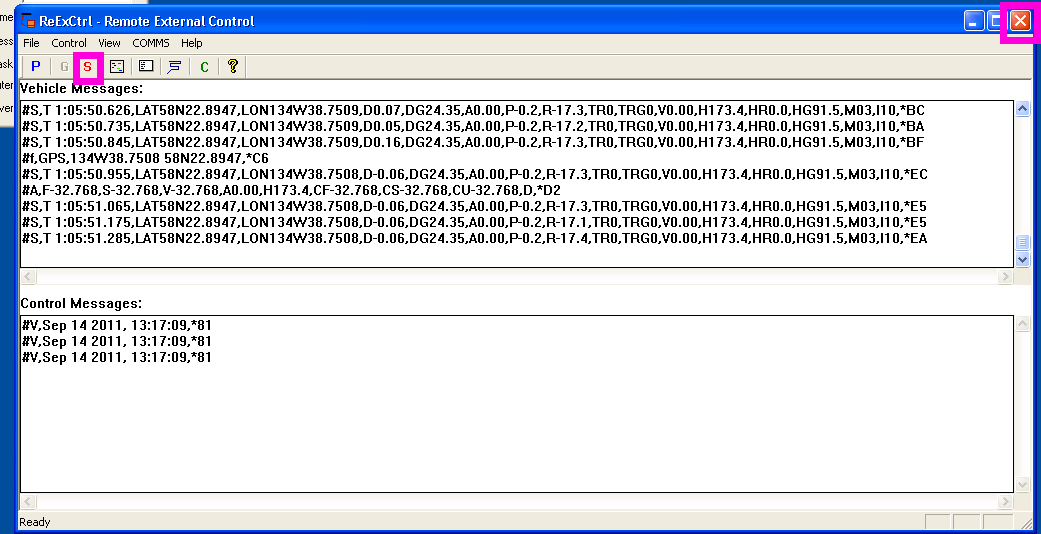
\includegraphics[width=0.95\textwidth]{img/remus_external_control.png}}
\caption{Stopping and closing REMUS External Control}
\label{fig:ext_control}
\end{figure}


\begin{figure}[h]
\centering{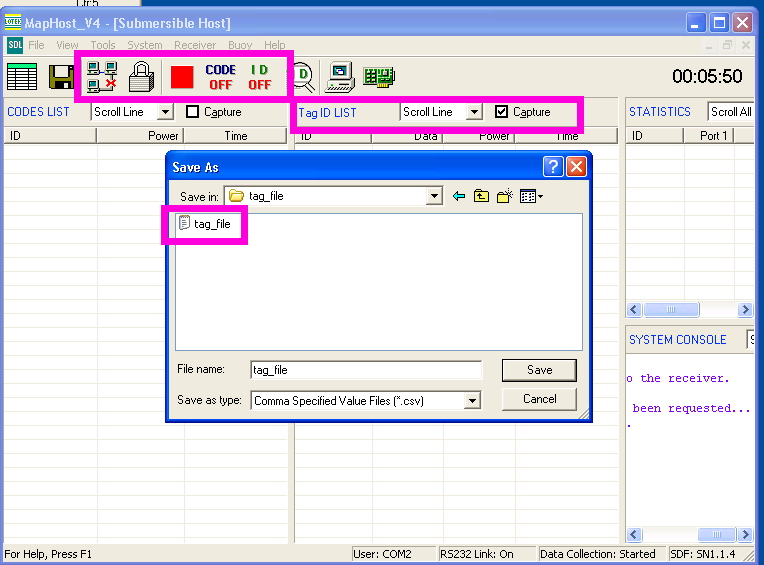
\includegraphics[width=0.95\textwidth]{img/tag_table.png}}
\caption{MapHost configuration}
\label{fig:maphost_setup}
\end{figure}

\begin{figure}[h]
\centering{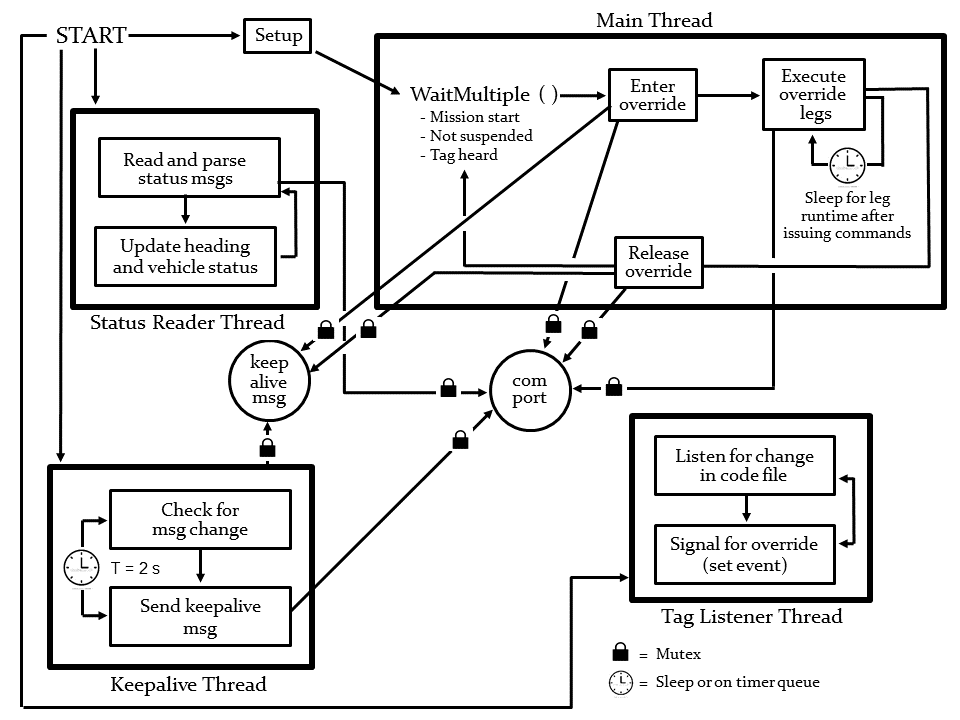
\includegraphics[width=0.95\textwidth]{img/SAOVR_Diagram.png}}
\caption{Control flow --- all threads.}
\label{fig:control_flow}
\end{figure}



\end{document}
